\documentclass[11pt,a4paper]{book} % Basisdokumentenklasse
\usepackage[ngerman]{babel}        % Deutsche Standardbezeichner und Trennung
%\usepackage[latin1]{inputenc}      % F\"{u}r Umlaute
\usepackage[T1]{fontenc}           % und {\ss}
\usepackage{makeidx}               % Indexpaket
\usepackage{times}                 % Sch\"{o}nere Schriften, Achtung, nicht pslatex verwenden!
\usepackage{longtable}             % Lange Tabelle f\"{u}r Abk\"{u}rzungsverzeichnis
\usepackage{graphics}              % EPS-Grafiken einbinden
\usepackage{hyperref}

\usepackage{fancyvrb}              % Fancy-Verbatin f\"{u}r Programmlistings


\usepackage{style/abtisstud}           % Das Abteilungs-Stylepaket, am Ende einbinden!



% Einstellungen f\"{u}r die "offizielle" Titelseite
\title{Anwendung des Style-Pakets\\[0.2em] f\"{u}r Arbeiten in LaTeX} % Titel der Arbeit
\author{Cinddy Vannessa Canon Pasquel} % Name des Autors
\date{Juni 2020}
\studiengang{Bachelorstudiengang Informatik}
\arbeitstyp{Bachelorarbeit}
\erstgutachter{ Dr. Ute Vogel-Sonnenschein}
\zweitgutachter{Prof. Dr. Zweiter Gutachter}

% Index erneuern
\makeindex

%\includeonly{content/kapitel1}

% Das eigentliche Dokument
\begin{document}
%Damit die Hyperrefs richtig funktionieren (vor allem bei Seite 1)
\pagenumbering{gobble}

% Anfang des Dokuments
\maketitle              % Offizielle Titelseite der Uni

\newpage
\thispagestyle{empty}
%\cleardoublepage

\pagenumbering{Roman}   % R\"{o}mische Seitenzahlen f\"{u}r den Anfang

% Zusammenfassung und Abstract
%\chapter*{Zusammenfassung}
Dieses Dokument repr�sentiert Struktur und Designvorlage des neuen
Abteilungsstils f�r studentische Arbeiten.



% Inhaltsverzeichnis
\renewcommand{\contentsname}{Inhalt} % Es soll nicht Inhaltsverzeichnis hei{\ss}en, sondern Inhalt
\tableofcontents        % Inhaltsverzeichnis einbinden
\cleardoublepage        % Danach auf ungerader Seite weitermachen
\pagenumbering{arabic}  % Arabische Seitenzahlen starten neu


% Der eigentliche Inhalt, hier k\"{o}nnte man dann auch jedes Kapitel einzeln einf\"{u}gen
\section{Einleitung}
Die Erstellung dieser Bachelorarbeit findet innerhalb des Studiengangs Informatik der Fakult\"at II - Informatik, Wirtschafts- und Rechtswissenschaften an der Carl von Ossietzky Universit\"at Oldenburg statt.
Dieses Expos\'{e} soll eine kurze Einleitung in die durchzuf\"uhrende Bachelorarbeit darstellen.\\

Im Folgenden m\"ochte ich eine grobe Einf\"uhrung in die Thematik geben, die Zielsetzung, die Motivation und die Problemstellung meiner Bachelorarbeit beschreiben, eine aktuelle \"Ubersicht vorhandener Studien darlegen und abschlie{\ss}end meine vorl\"aufige Gliederung und Zeitplanung vorstellen.
\section{Einfürung}
Die Struktur des Studienplans eines akademischen Bachelorprogramms an der Carl von Ossietzky Universität Oldenburg besteht aus vier verschiedenen Modulkategorien. Zum einen aus Basis- und Aufbaumodulen, die zu dem Pflichtbereich gehören und die wichtige Grundlage des Studiums vermitteln; zum zweiten aus Akzentssetzungsmodule, die Studierenden eine individuelle Ausrichtung geben können. Zusätzlich gibt es Professionalisierungs- und Praxismodule, die den Erwerb berufsbezogener und praktischer Kenntnisse stellen. Zulässt muss ein Abschlussmodul abgeschlossen werden. Master of Education und Master sind anderes aufgebaut aber auch für sie gibt es Abschlussarbeit.
Das Abschlussmodul ist eine vertiefende Prüfungsleitung, die von den Studenten als Voraussetzung für die Qualifikation des Abschlusses entwickelt wurde\cite{BScInf:2020}.\\

Bei der Anfertigung der Abschlussarbeit muss die\textbackslash der Studierende zunächst ein Thema für ihre\textbackslash seine Forschungsarbeit finden, welches für sein Studienprogramm relevant sein muss. Es ist möglich, dass Studierende in Absprache mit einer Gutachterin bzw. einem Gutachter selbst ein Thema für eine Abschlussarbeit wählen können, oder dass, es durch eine Einrichtung au{\ss}erhalb der Universität ausgeführt werden kann\cite{Boles:2015}.\\

Das Department für Informatik ist in vier Fachrichtungen aufgegliedert: Theoretische Informatik, Praktische Informatik, Angewandte Informatik und Technische Informatik, und jede davon ist nochmal in verschiedene Vertiefungsrichtungen unterteil. Insgesamt gibt es siebzehn Abteilungen\cite{SpeInf:2020}. Jede Abteilung setz sich aus Professoren und wissenschaftliche Mitarbeiter zusammen, die eine Forschungsgruppe bilden und für die von ihr durchgeführten Projekte verantwortlich sind.
Für Abschlussprojekte, die an der Universität entwickelt wurden, jede Abteilung des Departments für Informatik sollte, auf einer Abteilungs-eigenen Website, aktuelle Themen für Abschlussarbeiten veröffentlichen oder beschreiben, wie Studierende in der entsprechenden Abteilung ein Thema erhält\cite{Boles:2015}.\\

Der Zugang zu Informationen über die Abschlussthemen sollte von dem Department für Informatik gewährleistet werden, indem es eine standardisierte Form der Suche anbietet, welche den Universitätsmitarbeitern ermöglicht, die veröffentlichten Informationen effizient zu aktualisieren, und Studierende ermöglicht, ihre persönlichen Interessen zu berücksichtigen.

\newpage
\subsection{Zielsetzung}
Diese Bachelorarbeit beschäftigt sich gezielt mit der Themenfindung und Verwaltung von Abschlussarbeiten. In diesem Zusammenhang sollte klargestellt werden, welche Kriterien sind für die Suche nach einem Forschungsthema relevant und unter welchen Parametern kann der aktuelle Prozess der Veröffentlichung und Zuordnung von Abschlussarbeitsthemen optimiert werden. Diese Informationen werden für die Entwicklung und Implementierung einer Softwareanwendung berücksichtigt, mit der Studierende nach Themen von Abschlussarbeiten suchen und Mitarbeiter des Fachbereichs Informatik diese zuweisen und verfolgen können.

\section{Motivation}
Die Suche nach Abschlussthemen durch Studierende ist nicht einfach.  Das umfangreiche Angebot an Spezialisierungen bzw. Abteilungen des Departments für Informatik ermöglicht es den Studenten, sich mit dem Bereich zu befassen, der sie am meisten anspricht. Es gibt jedoch zahlreiche Forschungsthemen, die sogar zu verschiedenen Studienbereichen gehören können, wie bei Projekten der Abteilung Didaktik der Informatik - Fachgebiet Angewandte Informatik, wo Kenntnisse der Mikrorobotik / Regelungstechnik und Softwaretechnik, die Teil der Fachrichtungen Technische Informatik bzw. Praktische Informatik sind, erforderlich sein können.\\

Auf Grundlage der obigen Ausführungen werden die folgenden Fragestellungen aufgegriffen:

\begin{itemize}
	\item Welche Suchkriterien verwenden Studierende bei der Suche nach Abschlussarbeitsthemen in Begleitung mit wissenschaftlicher Mitarbeitern des Departments für Informatik?
	
	\item Welche Elemente sind für die Mitarbeitern des Departements für Informatik relevant, um die Verwaltung der zugewiesenen Projekte zu gewährleisten?
\end{itemize}

Diese Arbeit muss eine Lösung für die Probleme des Departments für Informatik bei der Suche, Zuordnung und Verwaltung von Abschlussarbeiten bieten. Basierend auf den Bedürfnissen von Studenten und akademischen Mitarbeitern und unter Verwendung der technologischen Werkzeuge, die die Universität anbietet.
\subsection{Problembeschreibung}
Derzeit posten die Abteilungen die verfügbaren Forschungsthemen, die als Abschlussarbeiten gelten können, in den Pinnwänden der Fakultätsbüros, sodass interessierte Studierende an der Universität sein müssen, um über diese Themen informiert zu werden.
Einige Abteilungen veröffentlichen die Themen zusätzlich auf der Website der Universität, es gibt eine zentrale Seite und da drunter Seiten für Abteilungen. Die Mitglieder der Abteilung müssen dann ständig auf die Aktualisierung der Projekte auf der Website achten aber nicht jeder Mitarbeiter hat Zugangsrechte auf die Aktualisierung des Inhalts der Website. Es ist nicht immer klar, welche Projekte bereits in Bearbeitung sind und welche noch verfügbar sind.\\

Andere Abteilungen wie Eingebettete Hardware- / Software-Systeme bitten an Studierende, die an Abschlussarbeitsthemen interessiert sind, eine formlose Bewerbung mit   den bisher belegten Modulen, persönlichen Kenntnissen und Interessen, an einen wissenschaftlichen Mitarbeiter der Abteilung zu senden. Dieser wird Ihnen dann mögliche Themen zukommen lassen und bei Bedarf einen Termin organisieren\cite{EHS:2020}.
Obwohl die Studierenden auf diese Weise eine persönliche Beratung erhalten, hängen die Antwortzeiten von der Verfügbarkeit der Mitarbeiter der Abteilung ab, und es kann sein, dass die angebotenen Projekte für den Studenten nicht von Interesse sind, was die Suche nach einem Forschungsthema weiterhin verzögern würde. Die Kommunikation erfolgt über Emails, die übersehen werden können und die nicht direkt zu einem Projekt verknüpft werden können, um die effektive Verwaltung der Abschlussarbeit zu gewährleisten.\\

Die aktuelle Art und Weise, in der die als Abschlussarbeit verfügbaren Forschungsthemen veröffentlicht werden, ermöglicht es den Studierenden nicht, eine schnelle, effiziente und personalisierte Suche entsprechend den Bedürfnissen der einzelnen Studierenden durchzuführen. Für die Mitarbeiter der Abteilung ist es derzeit nicht effizient, die Veröffentlichung verfügbarer Themen aufrechtzuerhalten und Informationsanfragen von Studenten weiterzuverfolgen.\\
Darüber hinaus hat das Department keinen Überblick darüber, wie viele Abschlussarbeiten derzeit angeboten werden und wie viele gesucht werden, sodass das Risiko besteht, dass sich der Abschluss der Studierenden durch eine lange Suchzeit verzögert.
\section{Stand der Forschung}
Im Bereich der Durchführung eines Studienprojekts wurde 2009\cite{Watat:2019} ein Lösungsvorschlag für das Problem der Suche nach Forschungsprojekten am DfI vorgelegt. Dieser Vorschlag wurde als Webanwendung konzipiert, die der Website der Universität hinzugefügt wurde. Dort müssen die Mitarbeiter der Abteilung Informationen aus Forschungsprojekten eingeben, die sowohl von Universitätsmitarbeitern als auch von externen Benutzern konsultiert werden können.
Die Webanwendung wurde mit HTML, CSS und Java sowie mit der MySQL-Datenbank programmiert. Die Suche erfolgt anonym, es erfolgt keine Authentifizierung.\\

Einige der Themen für Forschungsprojekte, die als Abschlussprojekte abgeschlossen werden können, werden derzeit auf der Website der Universität veröffentlicht. Die Informationen können öffentlich eingesehen werden, und da keine Authentifizierung vorliegt, ist es nicht möglich zu wissen, wie viele Personen an den Themen interessiert sind, oder zusätzliche Ma{\ss}nahmen zur Konsultation durchzuführen.\\

Die Universität nutzt die Stud.IP-Arbeitsumgebung, um die interne Kommunikation zwischen Fakultät und Studierenden zu verwalten. Dafür arbeiten die für die Verwaltung der Plattform zuständigen Mitarbeiter ständig an Tools und Funktionen, die die Benutzerinteraktion verbessern.
Stud.IP ist eine kostenlose, Open Source Softwareplattform, deren Hauptprogrammiersprache PHP ist\cite{SIPPHP:2020}. Unter diesen Merkmalen ist es möglich, die Software- und Programm-Widgets-Anwendungen als Ergänzung zur Hauptplattform herunterzuladen.\\
Als Open-Source-Software ist Stud.IP lizenzkostenfrei\cite{SIPOS:2020}, d.h. jeder kann sich die Software herunterladen, installieren und unbegrenzt nutzen. Entwickelt wird die Software von der Stud.IP-CoreGroup, der aktiven Entwicklungsgemeinschaft, einer Gemeinschaft von Betreibereinrichtungen, der data-quest GmbH sowie dem Hochschulverein ELAN e.V.\\

In letzter Zeit wurden Funktionen für die Stud.IP-Umgebung der Universität aufgenommen, mit denen Fragebögen (VIPs) und Umfragen (Stoodle) offen oder anonym durchgeführt werden können und deren Informationen zur Erstellung von Statistiken verwendet werden können. Diese Werkzeuge anderseits werden verwendet um die Anforderungen Studierenden und Mitarbeitern zu erheben, was zeigt, dass eine Ergänzung von Plugins möglich ist.
%\subsection{Aufgabenstellung}
In Anbetracht der Vorteile von Stud.IP, wo bereits eine Struktur installiert ist, welche die Authentifizierung von Benutzern verwaltet und deren Kommunikation ermöglicht, wird die Softwareanwendung als Stud.IP-Plugin entwickelt, das der Plattform hinzugefügt wird und von Benutzern je nach Profil verwendet werden kann: Tutor oder Dozent.\\

Für Benutzer mit einem Tutor-Profil wird eine Übersicht erstellt, in der sie abhängig von den ausgewählten Auswahlkriterien nach Abschlussarbeiten suchen können.

Benutzer mit einem Dozent-Profil verfügen über eine Übersicht, in der sie Abschlussarbeitsthemen hinzufügen, ändern oder löschen können.

\subsubsection{Vorläufige Datenstruktur}
Eine Fakultät kann mehrere Departments haben, jedes Department kann aber nur zu einer Fakultät gehören und es kann verschiedene Fachrichtungen besitzen.
Jede Fachrichtung kann nur zu einem Department zugeordnet werden und kann in mehrere Abteilungen unterteilt werden, wobei eine Abteilung nur zu einer Fachrichtung gehören kann.
Mehrere Betreuer können einer Abteilung zugehörig sein aber ein Betreuer ist jeweils nur einer Abteilung zugeordnet.\\

Ein Thema besteht aus einem Identifikator, einem Namen, einer Beschreibung und ein Veröffentlichungsdatum. Es wird in einer Sprache geschrieben und wird einer Forschungsart zugeordnet: praktisch oder theoretisch. Ebenso besitzt das Thema einen Wert für den Status, wie zum Beispiel reserviert oder in Bearbeitung. Au{ss}erdem werden für das Thema verschiedenen Kompetenzen vorausgesetzt, welche wiederum Voraussetzungen mehrerer Themen sein können.\\
Sollte sich eine Studierende für ein Thema interessieren, kann sie es reservieren. Daraufhin kann ihr das Thema von einem Dozenten zugeordnet werden.\\

Die vorläufige Entitäten und ihren Beziehungen werden in folgender Abbildung vorgestellt:\\


\cleardoublepage
\begin{figure}[hp]%[H]
    \centering
    %\textbf{Your title}\par\medskip
    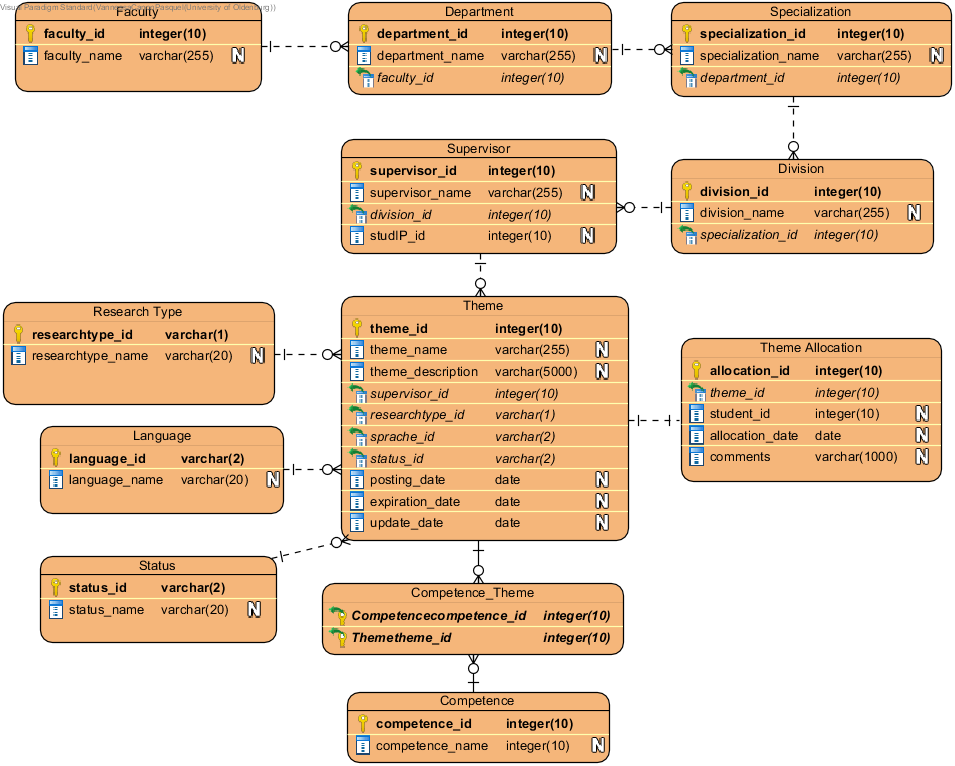
\includegraphics[height=12.5cm,keepaspectratio]{pics/ER_model}\\
    \caption{ER-Modell}
\end{figure}


\subsubsection{Definition von Suchkriterien}
Damit die Ergebnisse den Erwartungen der Studierenden so genau wie möglich entsprechen, wird eine Umfrage auf Basis der vorläufigen Datenstruktur durchgeführt.
In der Umfrage wird gefragt, welche Kriterien sind für die Studierenden relevant, wenn sie nach Themen für Abschlussarbeiten suchen und auch welche zusätzliche Funktionalitäten wären für die Softwareanwendung gewünscht.\\

\newpage
\textbf{Vorläufige Umfrage:}\\

Welche Kriterien sind für Sie relevant, bei der Suche nach Themen für Abschlussarbeiten:
	
	\begin{itemize}
	\item Studienabschluss
	\item Studiengang
	\item Fakultät
		\begin{itemize}[noitemsep]
			\item Department
			\item Fachrichtung
			\item Abteilung
			\item Betreuer
		\end{itemize}
	\item Forschungsart: Theoretisch, Praktisch
	\item Projekte ansehen
		\begin{itemize}[noitemsep]
			\item Verfügbare
			\item Reservierte
			\item Abgeschlossene
		\end{itemize}
	\item Angeforderte Kompetenzen: JAVA, SQL, Android, IoT, ERP{...}
	\item Sprache
	\item Veröffentlichungsdatum von - bis
	\item Ähnliche Projekte
	\item Andere:
	\end{itemize}
Gewünschte Funktionalitäten:
	
	\begin{itemize}
	\item Mehr Information über das Thema anfordern
	\item Projekt als Favorit merken
	\item Thema reservieren/befreien
	\begin{itemize}[noitemsep]
		\item Mehrere Projekte reservieren
		\item Projekte können von mehreren Studierenden reserviert werden
	\end{itemize}
	\item Andere:	
	\end{itemize}

\subsubsection{Entwurf der Softwareanwendung}
Benutzer können nach der Authentifizierung auf Stud.IP auf die Softwareanwendung-Plugin zugreifen.\\
Die Anwendung wird in PHP entwickelt, da dies die Hauptprogrammiersprache von Stud.IP ist.
Die Benutzeroberfläche enthält grafische Steuerelemente wie Button, Dropdown List, Text Box und Check Box, und es wird in ein Suchabschnitt im linken Bereich der Anwendung und ein Anzeigeabschnitt im rechten Bereich unterteilt, in dem die aus der Datenbank erhaltenen Ergebnisse gemä{\ss} den vom Benutzer ausgewählten Kriterien aufgelistet werden. Gruppen können zusammengeklappt und  aufgeklappt werden.\\

Wenn einen der Datensätze selektiert wird, werden zusätzliche Informationen zum ausgewählten Thema angezeigt, sodass der Benutzer das Abschlussarbeitsthema reservieren kann. Der Status des Themas wird in reserviert geändert, wodurch ein Datensatz in der Themenzuordnungstabelle generiert wird.\\
Die ausgewählten Filter, die Anzahl der abgerufenen Datensätze der Abfrage und eine Option zum Sortieren der Ergebnisse werden im Anwendungsheader angezeigt
Paginierung wird am Ende der Seite eingefügt, um eine gro{\ss}e Anzahl von Datensätzen zu unterstützen.\\

Die folgenden Bilder zeigen das vorläufige Design der Suche Übersicht. Anhang A enthält zusätzliche Bilder des Entwurfs nach dem Anwenden von Filtern.

\begin{figure}[hp]%[H]
    \centering
    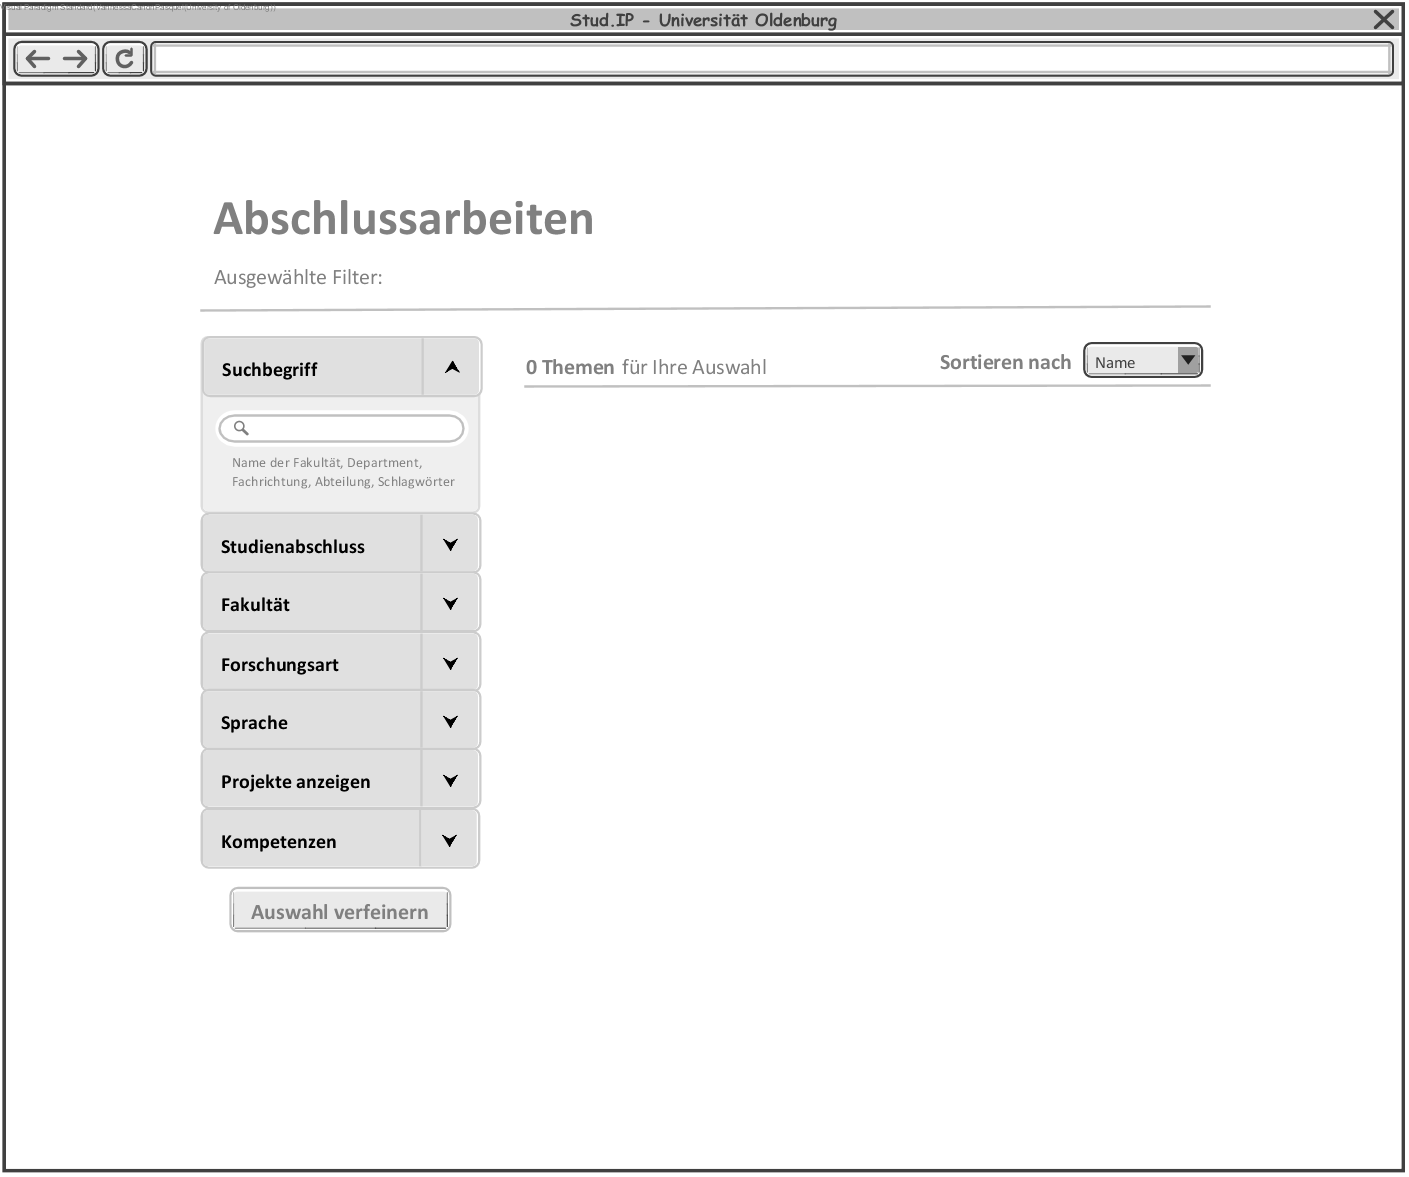
\includegraphics[height=7.5cm,keepaspectratio]{pics/app_collapsed}\\
    \caption{Suchkriterien zusammengeklappt}
\end{figure}

\cleardoublepage
\begin{figure}[hp]%[H]
    \centering
    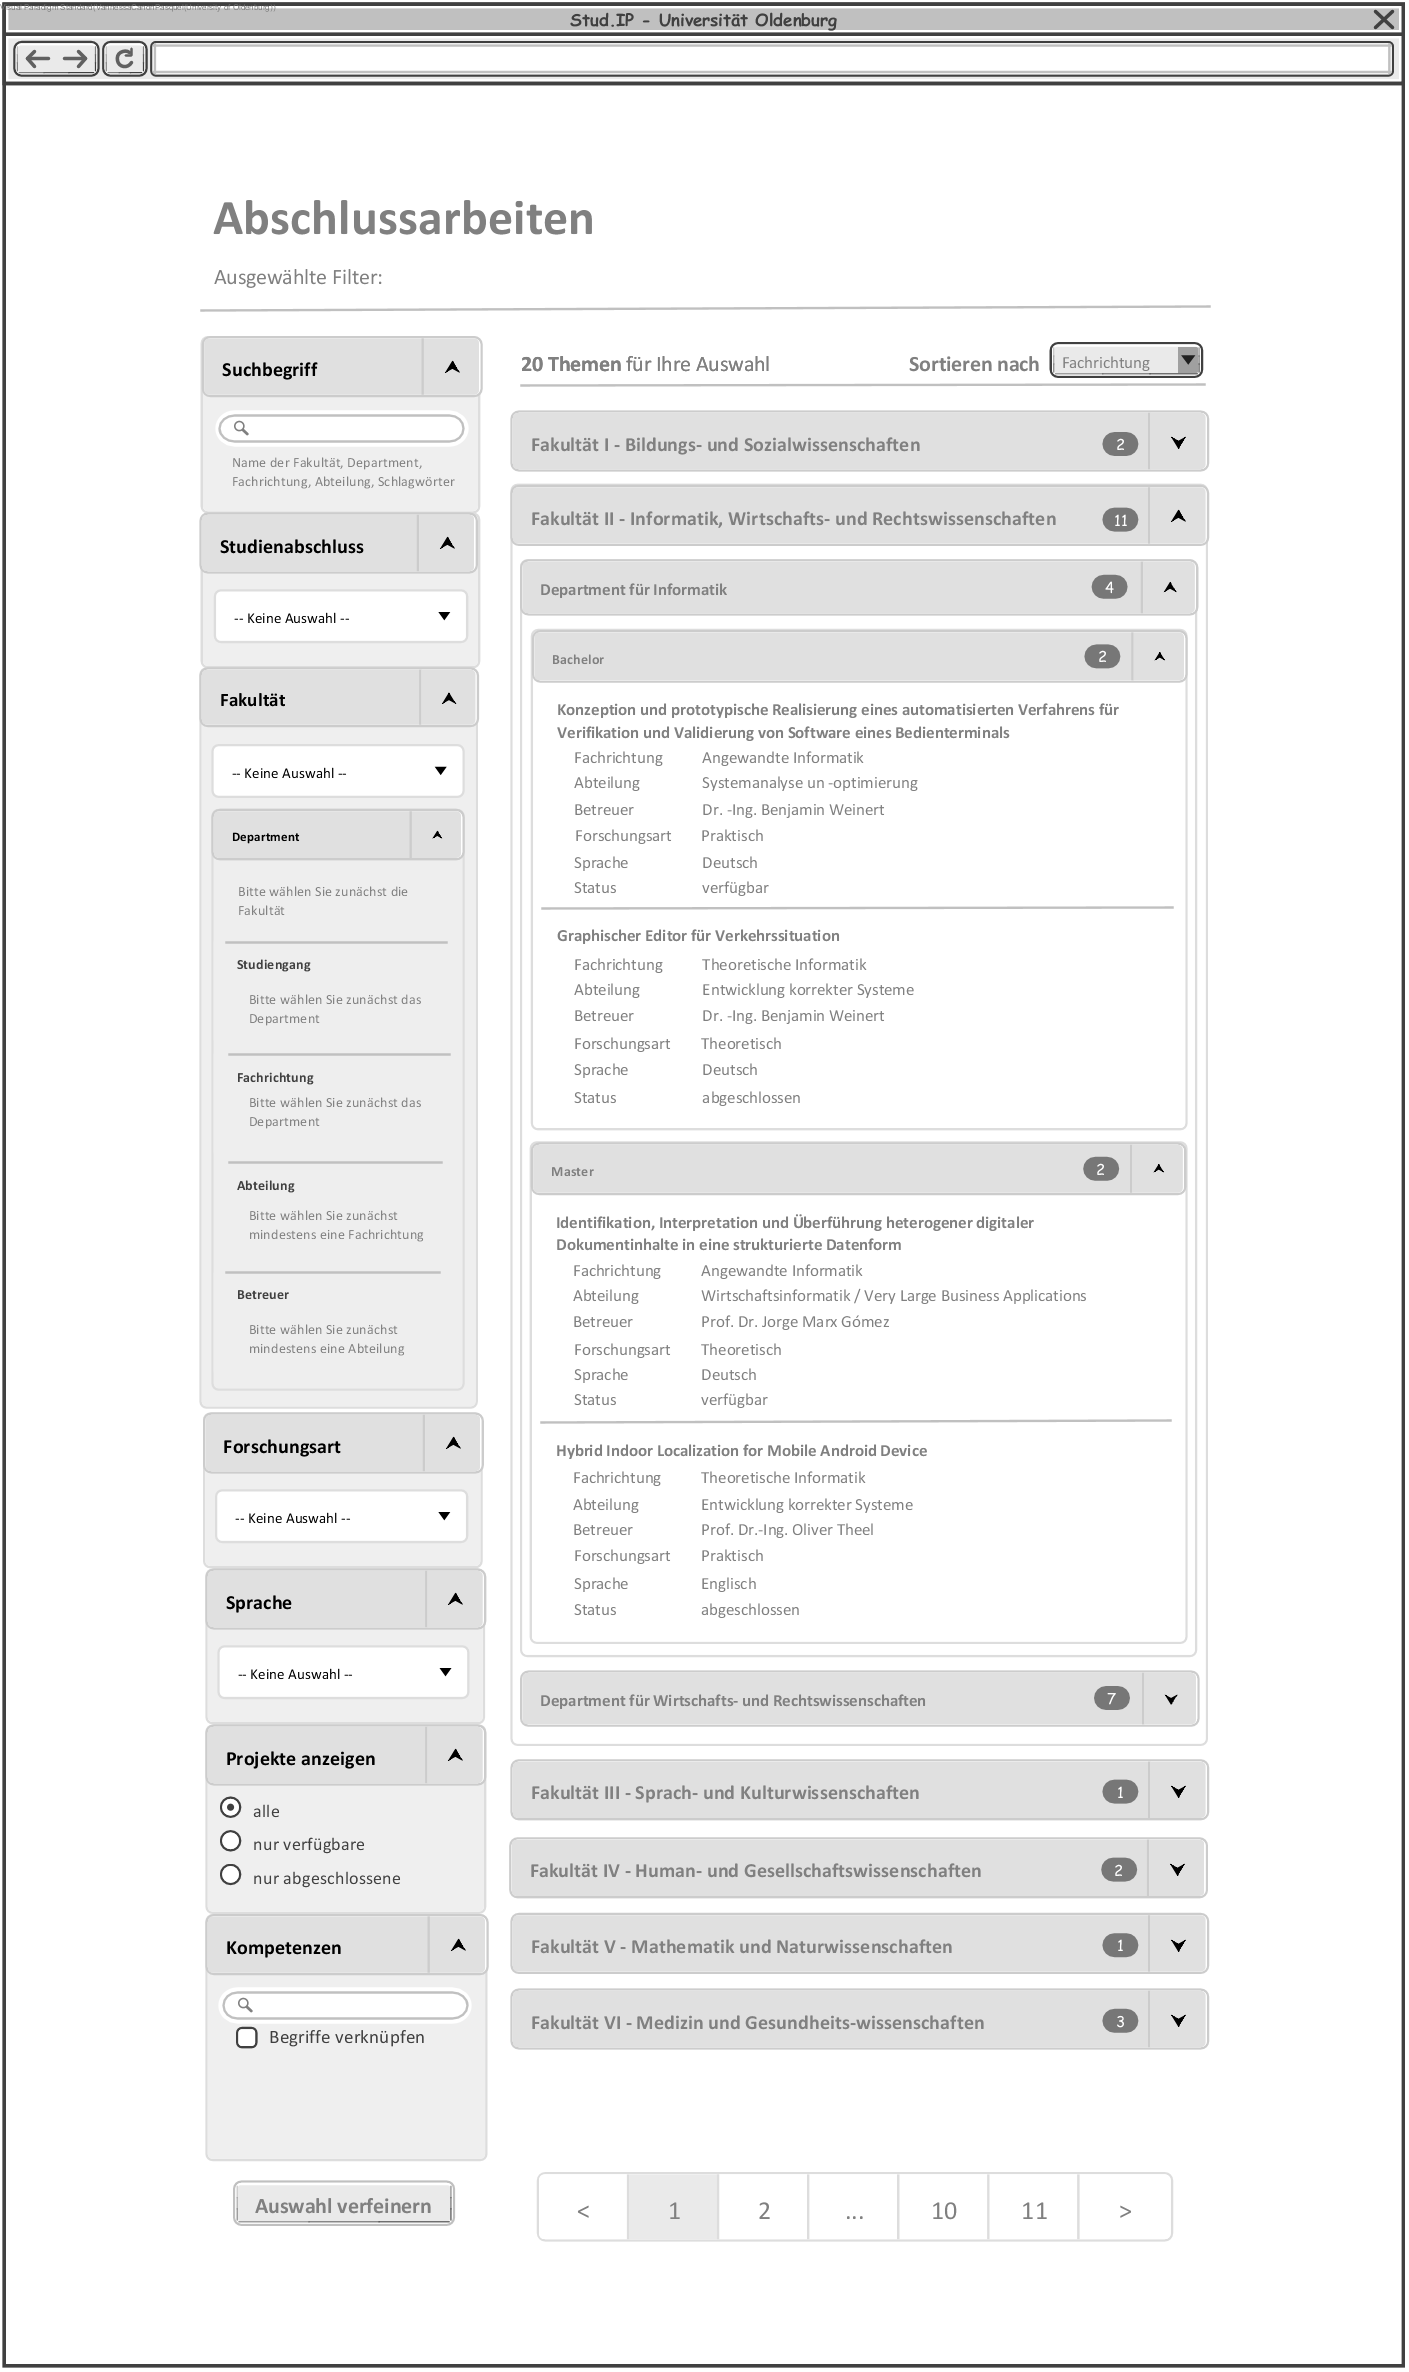
\includegraphics[height=20.5cm,keepaspectratio]{pics/app_expanded}\\
    \caption{Suchkriterien aufgeklappt - ohne Filter}
\end{figure}

\cleardoublepage
Zusätzlich wird eine Grundansicht für die Erstellung, Änderung und Beseitigung von Forschungsthemen durch Benutzer mit einem Dozent-Profil hinzugefügt. Dort werden Name, Beschreibung, Forschungsart, Sprache, Status und Ablaufdatum definiert. Nach der Erstellung wird das Veröffentlichungsdatum gespeichert.
Das Forschungsthema wird direkt der Abteilung des Benutzers zugewiesen, es kann jedoch definiert werden, wer der Betreuer ist.\\

Der Benutzer kann den Status des Themas ändern und festlegen, ob er akzeptiert, dass es von mehreren Benutzern reserviert werden kann, falls mehr als ein Benutzer an einem Thema interessiert ist, aber schließlich nur einer von ihnen es annehmen möchte. Ein Thema kann nur einem Benutzer zugewiesen werden.
Nachdem ein Thema geändert wurde, das Aktualisierungsdatum gespeichert.
  

%\section{Vorläufige Gliederung}

\begin{legal}[noitemsep]
\item Einleitung
	\begin{legal}
	\item Einführung und Zielsetzung
	\item Motivation
	\item Problembeschreibung
	\item Stand der Forschung
	\item Aufgabenstellung
	\end{legal}
\item Struktur des Departments für Informatik
	\begin{legal}
	\item Fachrichtungen
		\begin{legal}
		\item  Abteilungen
			\begin{legal}
			\item  Leitung
			\item  Betreuer
			\item  Veröffentlichung und Zuweisung von Abschlussarbeiten
			\end{legal}
		\end{legal}
	\end{legal}
\item Anforderungsanalyse
	\begin{legal}
	\item Ergebnisse der Umfrage und Datenanalyse
	\item User Stories
	\item Technische Anforderungen
	\item Definition der Suchkriterien und Suchalgorithmus
	\item Modellierung
		\begin{legal}
		\item  Entitäten und Beziehungen der Datenbank
		\item  Benutzeroberfläche
			\begin{legal}
			\item  Tutor
			\item  Dozent
			\end{legal}
		\end{legal}
	\end{legal}
\item Entwicklung und Implementierung
	\begin{legal}
	\item Herausforderungen
	\item Tests
	\item Ergebnisse
	\end{legal}
\item Fazit
\item Anhang
\item Literaturverzeichnis
Erklärung
\end{legal}
%\chapter{Vorläufige Zeitplanung}
gemäß den Leitfaden zur Durchführung von Bachelor-Abschlussarbeiten\cite{Boles:2015}, die Dauer der Bachelorarbeit beträgt vier Monate.\\
Der erste Teil der Zeit wird genutzt um das Projekt vollständig zu strukturieren. In der Einarbeitungsphase, wird das notwendige fehlende Wissen erworben.\\
Die dritte Phase befasst sich mit der Entwicklung der Softwareanwendung sowohl auf Datenbank- als auch auf Benutzeroberflächenebene sowie deren jeweiligen Tests.\\
In der Schreibphase, wird der Software-Quellcode wird dokumentiert, ein Benutzerhandbuch wird geschrieben und die schriftliche Ausarbeitung der Bachelorarbeit wird erstellt.
In der letzten Phase wird die Dokumentation vor der Abgabe überprüft und korrigiert, die Folien und Dokumente für den Vortrag werden geschrieben.

\begin{figure}[hp]%[H]
    \centering
    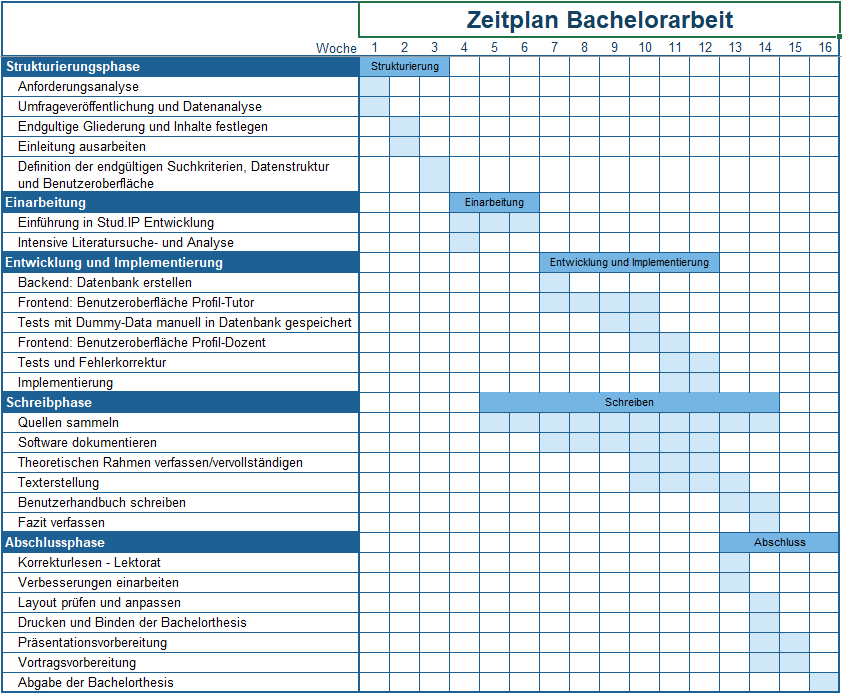
\includegraphics[height=12.5cm,keepaspectratio]{pics/zeitplan}\\
    \caption{Zeitplanung}
\end{figure}

%\section{Abzuliefernde Ergebnisse}
\begin{itemize}
	\item schriftliche Ausarbeitung der Bachelorarbeit
	\item CD-ROM mit:
	\begin{itemize}
		\item Programme
		\item Source-Code
		\item Benutzerhandbuch
		\item multimediale Supplementen
		\item Präsentationsfolien
	\end{itemize}
\end{itemize}

%\chapter{Anwendung des Style-Pakets} \index{Anwendung}
Nachfolgend ein kurzer Leitfaden f\"{u}r die Anwendung des
vorliegenden Style-Pakets f\"{u}r LaTeX-Dokumente f\"{u}r Arbeiten in der
Abteilung Informationssysteme

\begin{itemize}
\item Autor: Markus Schmees
\item Anpassungen f\"{u}r studentische Arbeiten: Marco Grawunder und Richard Hackelbusch
\item Version: 1.3.2
\item Stand: 24.04.2009
\end{itemize}

\section{Einbinden des Pakets}\index{Einbinden}\index{Paket}
Die einfachste M\"{o}glichkeit besteht darin, das vorgegebene Dokument
mit dem Titel

\texttt{BEARBEITER.tex}

zu verwenden und um eigene
Inhalte zu erg\"{a}nzen. BEARBEITER sollte durch die Art der Arbeit und den Namen des Autors ersetzt werden. Alternativ dazu kann der Autor im eigenen
\LaTeX-Hauptdokument, das die Dokumentenklasse \texttt{book}, eine
\texttt{11pt}-Schrift sowie die Blattgr\"{o}{\ss}e \texttt{a4paper}
verwenden muss, zus\"{a}tzlich am Ende der Paketdeklarationen das
Abteilungsstylepaket durch folgenden Befehl einbinden

\begin{verbatim}
\usepackage{abtisstud/abtisstud}
\end{verbatim}

Hierbei aber darauf achten, dass das Paket als \textbf{letztes
Paket} eingebunden wird, da es diverse \LaTeX-Befehle
\"{u}berschreibt, die von anderen Paketen ebenfalls \"{u}berschrieben
werden k\"{o}nnen. Das resultierende Hauptdokument sollte dann die in
der folgenden Abb.~\ref{stylepaket} dargestellte Struktur besitzen

\begin{figure}[ht]
\centering
\begin{Verbatim}[label=dissertation.tex,numberblanklines=false,fontsize=\scriptsize,numbers=left,frame=single]
\documentclass[11pt,a4paper]{book} % Basisdokumentenklasse
\usepackage[latin1]{inputenc}      % F\"{u}r Umlaute
\usepackage[T1]{fontenc}           % und {\ss}
\usepackage[ngerman]{babel}        % Deutsche Standardbezeichner und Trennung
\usepackage{makeidx}               % Indexpaket
\usepackage{times}                 % Sch\"{o}nere Schriften
\usepackage{longtable}             % Lange Tabelle f\"{u}r Abk\"{u}rzungsverzeichnis
\usepackage{graphics}              % EPS-Grafiken einbinden
\usepackage{abtisstud/abtisstud}   % Das Stylepaket am Ende einbinden!

% Das eigentliche Dokument
\begin{document}
... Inhalt ...
\end{document}
\end{Verbatim}
\caption{Einbinden des Style-Pakets}\label{stylepaket}
\end{figure}


\section{\"{A}nderungen gegen\"{u}ber \texttt{book}}\index{Anderungen@\"{A}nderungen}
Dem Erweiterungspaket zugrunde liegt der Dokumentenstil
\texttt{book}. Dieser wurde mit Hilfe des vorliegenden Pakets an
Besonderheiten der IS-Formatvorlage angepasst. Dabei wurden
folgende Dinge ver\"{a}ndert:

\begin{itemize}
\item Abschnittnummerierung auf Ebene 3 gesetzt (bis 1.1.1.1)
\item Auff\"{u}hrung im Inhaltsverzeichnis bis Ebene 1 (bis 1.1)
\item R\"{a}nder, Header, Textweite und Texth\"{o}he angepasst
\item Linken Einzug um 0,37cm bei neuem Absatz eingef\"{u}gt
\item Abstand der Abs\"{a}tze auf 6pt eingestellt
\item Seitenzahlen und Abschnitte im Header dargestellt
\item Abstand der \"{U}berschriften zum Text eingestellt
\item Farbe und Schrift der \"{U}berschriften festgelegt
\item Verzeichnisdeklarationen f\"{u}r korrekte Headeranzeige
\"{u}berschrieben
\item Abstand der Abbildungen zu den Unterschriften angepasst
\item Schriftart und Style f\"{u}r Abbildungsunterschriften
eingestellt
\item "`Offizielle"' Titelseite integriert
\item Seitenzahltypen (r\"{o}misch und arabisch) kombiniert
\item Fu{\ss}noten linksb\"{u}ndig und mit Abstand zwischen Nummer und
Text
\item S\"{a}mtliche Listen linksb\"{u}ndig
\item Geringere Einr\"{u}ckung der Unterstichpunkte im Index
\item Umwandlung der \"{U}berschriften f\"{u}r Verzeichnisse in
gleichwertige \"{U}berschriften ohne "`-ver\-zeich\-nis"'
\end{itemize}


\section{Einbinden von Abbildungen}\index{Abbildungen}
\index{Abbildungen}
\index{Einbinden!Abbildungen}
Wie bei der normalen Verwendung von \LaTeX{} k\"{o}nnen auch hier \"{u}ber
die entsprechenden Zusatzpakete Grafiken eingebunden werden. Immer
darauf achten, dass diese als Vektorgrafiken vorliegen, damit sie
problemlos skaliert und damit auch ohne Qualit\"{a}tsverlust gedruckt
werden k\"{o}nnen. Nachfolgend zeigt Abb.~\ref{abbildung} am Beispiel
des Uni-Logos, wie eine Abbildung eingebunden und angezeigt werden
kann (vlg. dazu auch Abschnitt \ref{Schriften}).

\begin{figure}[ht]
  \centering
  
\includegraphics[scale=1]{style/unilogo.pdf}
  \caption{Eine sch\"{o}ne Abbildung}\label{abbildung}
\end{figure}


\section{Erstellen und Anpassen des Indexes}\index{Indexerstellung}
Um das grundlegende Indexfile zu erzeugen, muss der Befehl
\texttt{makeindex} innerhalb des Haupt-\LaTeX-Dokuments aufgef\"{u}hrt sein.
Dieser erzeugt aus s\"{a}mtlichen \texttt{index}-Befehlen die Datei

\texttt{dissertation.idx}.

Um diese Datei ebenfalls passend zu
formatieren, wurde ein entsprechendes Stylefile namens

\texttt{abtisstud.ist}

erstellt. Die Anwendung dieses Styles auf den
Index erfolgt mit Hilfe des folgenden Befehls

\begin{verbatim}
makeindex -s abtisstud/abtisstud.ist -o content/index.tex \
    dissertation.idx
\end{verbatim}

Dieser Befehl sorgt daf\"{u}r, dass die Indexdaten entsprechend
formatiert und in die Datei \texttt{index.tex} in das Verzeichnis
\texttt{content} abgelegt werden. Von dort kann der neue Index
dann problemlos per input eingelesen werden. Also bitte nicht den
traditionell erzeugten Index \"{u}ber den Befehl
\texttt{printindex} einbinden! Der Auszug aus dem
\LaTeX-Hauptdokument zur Erzeugung und Einbindung des Indexes sieht
folgenderma{\ss}en aus

\begin{figure}[ht]
\centering
\begin{Verbatim}[label=dissertation.tex,numberblanklines=false,fontsize=\scriptsize,numbers=left,frame=single]
...

% Indexdatei erzeugen
\makeindex

% Das eigentliche Dokument
\begin{document}

...

\index{Irgendwas}                     % Einstufiger Indexeintrag
\index{Irgendwas!Ganzanderes}         % Zweistufiger Indexeintrag

...

% Index als letztes Verzeichnis
\cleardoublepage                      % Auf ungerader Seite beginnen
\addcontentsline{toc}{chapter}{Index} % Index im Inhaltsverzeichnis anzeigen
\begin{theindex}
{\indexfrontskip\Large\sffamily\bfseries\hfill A\hfill}\nopagebreak
 
  \item Abbildungen\dotfill 2
  \item \"Anderungen\dotfill 2
  \item Anwendung\dotfill 1

  \indexspace
{\indexfrontskip\Large\sffamily\bfseries\hfill E\hfill}\nopagebreak
 
  \item Einbinden\dotfill 1
    \subitem Abbildungen\dotfill 2

  \indexspace
{\indexfrontskip\Large\sffamily\bfseries\hfill F\hfill}\nopagebreak
 
  \item Festlegungen\dotfill 7

  \indexspace
{\indexfrontskip\Large\sffamily\bfseries\hfill I\hfill}\nopagebreak
 
  \item Indexerstellung\dotfill 3
  \item Internationalisierung\dotfill 4

  \indexspace
{\indexfrontskip\Large\sffamily\bfseries\hfill L\hfill}\nopagebreak
 
  \item Literatur\dotfill 7
  \item Literaturreferenzen\dotfill 7

  \indexspace
{\indexfrontskip\Large\sffamily\bfseries\hfill P\hfill}\nopagebreak
 
  \item Paket\dotfill 1

  \indexspace
{\indexfrontskip\Large\sffamily\bfseries\hfill S\hfill}\nopagebreak
 
  \item Schriften\dotfill 5

  \indexspace
{\indexfrontskip\Large\sffamily\bfseries\hfill T\hfill}\nopagebreak
 
  \item Titelseite\dotfill 8

  \indexspace
{\indexfrontskip\Large\sffamily\bfseries\hfill V\hfill}\nopagebreak
 
  \item Verzeichnisreihenfolge\dotfill 7

  \indexspace
{\indexfrontskip\Large\sffamily\bfseries\hfill Z\hfill}\nopagebreak
 
  \item Zitate\dotfill 7

\end{theindex}
             % Formatierten Index einbinden
\end{document}
\end{Verbatim}
\caption{Index erstellen, formatieren und integrieren}\label{indexintegration}
\end{figure}


\section{Internationalisierung}\index{Internationalisierung}
Durch Einbinden entsprechender Sprachpakete wird \LaTeX{} an
Besonderheiten bestimmter Sprachr\"{a}ume, z.B. deren Trennung oder
Verzeichnisbezeichnung angepasst. Durch die individuelle
Gestaltung bestimmter Verzeichnisnamen wurden die zugeh\"{o}rigen
Befehle aber \"{u}berschrieben. Das bedeutet nun, dass der vorliegende
Stil zwar problemlos f\"{u}r deutsche Arbeiten anwendbar ist, aber
diese Verzeichnisbezeichnung f\"{u}r Dissertationen in fremder Sprache
angepasst werden m\"{u}ssen. Diese betreffen also insbesondere die
folgenden Paket- und Verzeichnisdeklarationen in den Zeilen 3, 11,
14, 18, 19, 23, 25, 29 und 30.

\begin{figure}[htp]
\centering
\begin{Verbatim}[label=dissertation.tex,numberblanklines=false,fontsize=\scriptsize,numbers=left,frame=single]
\documentclass[11pt,a4paper]{book}

...

\usepackage[ngerman]{babel}

...

\usepackage{abtisstud/abtisstud}

...

% Das eigentliche Dokument
\begin{document}

...

% Verzeichnisse am Ende, erst das Glossar
\addonchapter{Glossar} %
Nachfolgend sind noch einmal wesentliche Begriffe dieser Arbeit
zusammengefasst und erl�utert. Eine ausf�hrliche Erkl�rung findet
sich jeweils in den einf�hrenden Abschnitten sowie der jeweils
darin angegebenen Literatur. Das im Folgenden im Rahmen der
Erl�uterung verwendete Symbol \this bezieht sich jeweils auf den
im Einzelnen vorgestellten Begriff, das Symbol \siehe{} verweist
auf einen ebenfalls innerhalb dieses Glossars erkl�rten Begriff.

\begin{description}
\item[Auktion] Eine \this ist das im \siehe{E-Commerce} am
H�ufigsten eingesetzte Verfahren zur dynamischen
\siehe{Preisfindung}. Interessenten k�nnen dabei durch Abgabe von
Geboten Preis, Dauer und Gewinner beeinflussen. Bei einer offenen
\this sind Bieter, H�he der Gebote und der aktuelle Preis f�r
alle Teilnehmer sichtbar, bei der geschlossenen (sealed) \this
erfolgt nur eine interne Benachrichtigung. Die bekanntesten Typen
sind die traditionelle \siehe{Versteigerung} sowie die
\siehe{holl�ndische}, \siehe{umgekehrte} und \siehe{verdeckte} \this.

\item[Behaviorismus] Der \this ist eine \siehe{Lerntheorie}, die
davon ausgeht, dass Wissen als Struktur unabh�ngig vom
\siehe{Lernenden} existiert und dass sein Verhalten operant
konditioniert ist, d.h. dass es als Konsequenz aus anderen
Verhaltensweisen resultiert. Erfolgt eine positive Reaktion,
beh�lt der \siehe{Lernende} neu erlerntes Verhalten bei, negative
Reaktionen f�hren zu einer Verminderung dieses Verhaltens. Der
\siehe{Lehrende} bestimmt dabei das zu erlernende Wissen und
ist f�r die Steuerung des \siehe{Lernprozesses} zust�ndig.
\end{description}


% Dann die Abk\"{u}rzungen
\addonchapter{Abk\"{u}rzungen}
\begin{longtable}[ht]{ll}
ADDIE & Analysis, Design, Development, Implementation, Evaluation\\  %E-Learning
ADEPT & Advanced Decision Environment for Process Tasks\\  %Konzept
ADL & Advanced Distributed Learning Initiative\\  %E-Learning
AGB & Allgemeine Gesch�ftsbedingungen\\  %Konzept
AGOF & Arbeitsgemeinschaft Online Forschung\\  %Einleitung
AICC & Aviation Industry Computer Based Training Committee\\  %E-Learning
API & Application Programming Interface\\  %TEL, Konzept
%ARIADNE & Alliance of Remote Instructional Authoring and Distribution Networks for Europe\\  %E-Learning
ARIS & Architektur integrierter Informationssysteme\\  %Konzept
ASC & Accredited Standards Committee\\  %EC-Grundlagen
ASP & Application Service Providing\\  %Integration
ASTD & American Society for Training and Development\\  %E-Learning
AXIS & Apache eXtensible Interaction System\\  %Implementierung
B2B & Business-to-Business\\  %Konzept, Glossar
B2C & Business-to-Consumer\\  %Konzept, Glossar
BDSG & Bundesdatenschutzgesetz\\  %EC-Grundlagen
BGB & B�rgerliches Gesetzbuch\\  %Konzept
BITKOM & Bundesverband Informationswirtschaft, Telekommunikation und neue Medien\\  % Grundlagen E-Commerce
BMBF & Bundesministerium f�r Bildung und Forschung\\  %Einleitung
BME & Bundesverband Materialwirtschaft, Einkauf und Logistik\\  %EC-Grundlagen
BPEL4WS & Business Process Execution Language for Web Services\\  %Implementierung
BSCW & Basic Support for Cooperative Work\\  %E-Learning
BSI & Bundesamt f�r Sicherheit in der Informationstechnik\\ %Literatur
CAL & Computer Aided/Assisted Learning\\  %E-Learning
CBT & Computer Based Training\\  %E-Learning, Vorgaben
CC & Creative Commons\\  %Konzept
CD & Compact Disc\\  %E-Learning
CELab & Labor f�r Content Engineering\\  %TEL
CMI & Computer Managed Instruction\\  %E-Learning
CMS & Content Management System\\  %TEL, Konzept
CORBA & Common Object Request Broker Architecture\\  %Konzept
CPU & Central Processing Unit\\  %Konzept
CSCL & Computer Supported Collaborative Learning\\  %E-Learning
CSCW & Computer Supported Cooperative Work\\  %TEL
CSS & Customer Support Services\\  %Konzept
CRM & Customer Relationship Management\\  %Konzept
CUL & Computerunterst�tztes Lernen\\  %E-Learning
DBMS & Datenbankmanagementsystem\\  %Konzept
DCOM & Distributed Component Object Model\\  %Konzept
DFN & Deutsches Forschungsnetz\\  %E-Learning
DIN & Deutsches Institut f�r Normung\\  %Lernen, E-Learning, TEL
DREL & Digital Rights Expression Language\\  %Konzept
DRM & Digital Rights Management\\  %Konzept
DVD & Digital Video Disc\\  %E-Learning
E2B & Education-to-Business\\  %Integration
E2C & Education-to-Consumer\\  %Integration
E2E & Education-to-Education\\  %Integration
EAI & Enterprise Application Integration\\  %Konzept
EAN & European Article Numbering\\  %Grundlagen-EC-Standards
EBPP & Electronic Bill Presentment and Payment\\  %Konzept
ebXML & Electronic Business Extensible Markup Language\\ %EC-Grundlagen
ECA & Event-Condition-Action\\  %Vorgaben
EC & Electronic Cash\\  %EC-Grundlagen, Konzept
ECC & E-Learning Courseware Certification\\  %E-Learning
EDI & Electronic Data Interchange\\  %EC-Grundlagen
EDIFACT & EDI for Administration, Commerce and Transport\\  %Konzept
EFQM & European Foundation for Quality Management\\  %TEL
EGBGB & Einf�hrungsgesetz zum B�rgerlichen Gesetzbuch\\  %Konzept
EITO & European Information Technology Observatory\\  % Grundlagen E-Commerce
ELAN & E-Learning Academic Network Niedersachsen\\  %Einleitung, Vorgaben
\end{longtable}


% Weiter mit Abbildungen
\cleardoublepage
\addcontentsline{toc}{chapter}{Abbildungen}
\renewcommand{\listfigurename}{Abbildungen}
\listoffigures

% Schlie{\ss}lich Literatur
\cleardoublepage
\addcontentsline{toc}{chapter}{Literatur}
\bibliographystyle{alphadin}
\renewcommand{\bibname}{Literatur}
\bibliography{content/bibliographie}

% Und ganz am Ende der Index
\cleardoublepage
\addcontentsline{toc}{chapter}{Index}
\begin{theindex}
{\indexfrontskip\Large\sffamily\bfseries\hfill A\hfill}\nopagebreak
 
  \item Abbildungen\dotfill 2
  \item \"Anderungen\dotfill 2
  \item Anwendung\dotfill 1

  \indexspace
{\indexfrontskip\Large\sffamily\bfseries\hfill E\hfill}\nopagebreak
 
  \item Einbinden\dotfill 1
    \subitem Abbildungen\dotfill 2

  \indexspace
{\indexfrontskip\Large\sffamily\bfseries\hfill F\hfill}\nopagebreak
 
  \item Festlegungen\dotfill 7

  \indexspace
{\indexfrontskip\Large\sffamily\bfseries\hfill I\hfill}\nopagebreak
 
  \item Indexerstellung\dotfill 3
  \item Internationalisierung\dotfill 4

  \indexspace
{\indexfrontskip\Large\sffamily\bfseries\hfill L\hfill}\nopagebreak
 
  \item Literatur\dotfill 7
  \item Literaturreferenzen\dotfill 7

  \indexspace
{\indexfrontskip\Large\sffamily\bfseries\hfill P\hfill}\nopagebreak
 
  \item Paket\dotfill 1

  \indexspace
{\indexfrontskip\Large\sffamily\bfseries\hfill S\hfill}\nopagebreak
 
  \item Schriften\dotfill 5

  \indexspace
{\indexfrontskip\Large\sffamily\bfseries\hfill T\hfill}\nopagebreak
 
  \item Titelseite\dotfill 8

  \indexspace
{\indexfrontskip\Large\sffamily\bfseries\hfill V\hfill}\nopagebreak
 
  \item Verzeichnisreihenfolge\dotfill 7

  \indexspace
{\indexfrontskip\Large\sffamily\bfseries\hfill Z\hfill}\nopagebreak
 
  \item Zitate\dotfill 7

\end{theindex}


% Und schlie{\ss}lich noch die Versicherung f\"{u}r das Pr\"{u}fungsamt
\cleardoublepage
\versicherung{Oldenburg}

\end{document}
\end{Verbatim}
\caption{Anzupassende Pakete bzw. Verzeichnisbezeichner}\label{verzeichnisanpassung}
\end{figure}




\section{Einbetten s\"{a}mtlicher Schriften}\index{Schriften}\label{Schriften}
Bitte unbedingt folgende Dokumenteneinstellung beibehalten

\begin{verbatim}
\documentclass[11pt,a4paper]{book}
\end{verbatim}

Grunds\"{a}tzlich bietet es sich an, die Arbeit mit \texttt{pdflatex} direkt als PDF zu erzeugen. Bei der Verwendung von \texttt{pdflatex} k\"{o}nnen als Bildformate PDF, PNG oder JPG (Achtung: Die beiden letzteren sind nicht im Vektorformat und damit nicht gut f\"{u}r den Ausdruck geeignet.) f\"{u}r Bilder verwendet werden.

Es sollten aber s\"{a}mtliche verwendete Schriftarten in das
resultierende PDF-Do\-kument eingebettet werden. \texttt{pdflatex}
und \texttt{ps2pdf} sparen unter Umst\"{a}nden einige Schriften aus, sollten also nur mit Bedacht verwendet werden.

Eine M\"{o}glichkeit, dennoch s\"{a}mtliche Schriftarten in das
resultierende Dokument einzubetten, bietet eine Kombination aus
\texttt{dvips} und \texttt{ghostscript} an. Zun\"{a}chst das
resultierende DVI-Dokument \texttt{dissertation.dvi} in ein
passendes PS-Dokument umwandeln mit dem folgenden Befehl

\begin{verbatim}
dvips -P pdf -t A4 -z -Pdownload35 dissertation.dvi
\end{verbatim}

Die resultierende Datei \texttt{dissertation.ps} darf daraufhin
NICHT mit
\texttt{ps2pdf} sondern muss -- wie der folgende Befehl zeigt --
mit \texttt{ghostscript} in ein PDF umgewandelt werden

\begin{verbatim}
gs -dSAFER -dNOPAUSE -dBATCH -sDEVICE=pdfwrite \

   -sPAPERSIZE=a4 -dPDFSETTINGS=/printer \

   -dCompatibilityLevel=1.3 -dMaxSubsetPct=100 \

   -dSubsetFonts=true -dEmbedAllFonts=true \

   -sOutputFile=dissertation.pdf dissertation.ps
\end{verbatim}

Das hieraus resultierende PDF-Dokument \texttt{dissertation.pdf}
enth\"{a}lt schlie{\ss}lich sowohl das gew\"{u}nschte Format als auch
s\"{a}mtliche Schriften. Bei dem Umweg \"{u}ber EPS ist allerdings zu beachten, dass Vektorgraphiken nicht als PDF sondern als EPS-Dateien eingebunden werden m\"{u}ssen.

\chapter{Festlegungen der Abteilung}\index{Festlegungen}
\"{U}ber das reine Design hinaus sind nachfolgend Festlegungen zur
Struktur einer Arbeit (insbesondere Studentischer Arbeiten) der
Abteilung Informationssysteme  aufgef\"{u}hrt.



\section{Verzeichnisreihenfolge}\index{Verzeichnisreihenfolge}
Die Reihenfolge der Verzeichnisse soll dem vorliegenden Dokument
folgen, die Verzeichnisse dazu wie folgt angeordnet sein. Im
Inhaltsverzeichnis, das neuerdings nur noch "`Inhalt"' hei{\ss}t,
werden nur die nachfolgend fett dargestellten Punkte aufgef\"{u}hrt.

\begin{enumerate}
\item Zusammenfassung
\item Abstract
\item Inhalt (vormals Inhaltsverzeichnis)
\item \textbf{Der eigentliche Inhalt} mit laufenden Kapitelnummern
\item \textbf{Glossar} und Folgende jeweils ohne Kapitelnummer
\item \textbf{Abk\"{u}rzungen}
\item \textbf{Abbildungen}
\item \textbf{Literatur}
\item \textbf{Index}
\end{enumerate}


Hierbei wurde auf die traditionelle Verwendung der Begriffe
Inhaltsverzeichnis, Literaturverzeichnis und Abbildungsverzeichnis
verzichtet und stattdessen nur noch Inhalt, Literatur und
Abbildungen verwendet.


\section{Zitate und Literaturreferenzen}\index{Zitate}\index{Literaturreferenzen}\index{Literatur}
Im eigentlichen Text kann man verschiedene Zitate verwenden. Das
machen auch z.B. \cite{abel03}, \cite{appelrath06}, \cite{back01}
oder \cite{bakos91}. Den jeweiligen Zitaten soll dazu der
Bibliographiestil \texttt{alphadin} (mit kleinem "`a"') zugrunde
liegen. Dieser repr\"{a}sentiert einen genormten Zitierstil und wird
durch folgende Zeile im \LaTeX-Dokument eingestellt

\begin{verbatim}
\bibliographystyle{alphadin}
\end{verbatim}

Wer trotz des verk\"{u}rzten Zitierstils in ausf\"{u}hrlicher Weise auf
die jeweiligen Autoren hinweisen m\"{o}chte, hat die M\"{o}glichkeit, dies
z.B. folgenderma{\ss}en zu machen: "`wie auch von Appelrath, Boles,
Kleinefeld und andere in
\cite{appelrath06} beschrieben\ldots"'

Bei den Literaturangaben wird k\"{u}nftig auf die ISBN- bzw.
ISSN-Nummern verzichtet, da bei Dissertationen ohnehin davon
auszugehen ist, dass begutachtete bzw. verlegte Literatur
verwendet wird.


\section{Die offizielle Titelseite}\index{Titelseite}
Der \texttt{maketitle}-Befehl wurde \"{u}berschrieben. F\"{u}r die neue Titelseite
sind daher folgende Einstellungen zu machen

\begin{figure}[ht]
\centering
\begin{Verbatim}[label=dissertation.tex,numberblanklines=false,fontsize=\scriptsize,numbers=left,frame=single]
% Voreinstellungen f\"{u}r offizielle Titelseite
\title{Hier den Titel einf\"{u}gen}                   % Titel der Dissertation
\author{Dipl.-Inform. Vorname Nachname}           % Name des Autors
\arbeitstyp{Diplomarbeit}                         % oder Bachelorarbeit, Masterarbeit ...
\erstgutachter{Prof. Dr. Erster Gutachter}        % Name des Erstgutachters
\zweitgutachter{Prof. Dr.-Ing. Zweiter Gutachter} % Name des Zweitgutachters

% Einbinden/Anzeigen der Titelseite innerhalb von \begin/end{document}
\maketitle
\end{Verbatim}
\caption{Einstellungen f\"{u}r offizielle Titelseite}\label{titelseite}
\end{figure}

%\chapter{Einleitung} \index{einleitung}

%\chapter{Einleitung} \index{einleitung}


% Verzeichnisse am Ende, erst das Glossar
\addonchapter{Glossar} % Es soll auch Glossar hei{\ss}en
%Nachfolgend sind noch einmal wesentliche Begriffe dieser Arbeit
zusammengefasst und erl�utert. Eine ausf�hrliche Erkl�rung findet
sich jeweils in den einf�hrenden Abschnitten sowie der jeweils
darin angegebenen Literatur. Das im Folgenden im Rahmen der
Erl�uterung verwendete Symbol \this bezieht sich jeweils auf den
im Einzelnen vorgestellten Begriff, das Symbol \siehe{} verweist
auf einen ebenfalls innerhalb dieses Glossars erkl�rten Begriff.

\begin{description}
\item[Auktion] Eine \this ist das im \siehe{E-Commerce} am
H�ufigsten eingesetzte Verfahren zur dynamischen
\siehe{Preisfindung}. Interessenten k�nnen dabei durch Abgabe von
Geboten Preis, Dauer und Gewinner beeinflussen. Bei einer offenen
\this sind Bieter, H�he der Gebote und der aktuelle Preis f�r
alle Teilnehmer sichtbar, bei der geschlossenen (sealed) \this
erfolgt nur eine interne Benachrichtigung. Die bekanntesten Typen
sind die traditionelle \siehe{Versteigerung} sowie die
\siehe{holl�ndische}, \siehe{umgekehrte} und \siehe{verdeckte} \this.

\item[Behaviorismus] Der \this ist eine \siehe{Lerntheorie}, die
davon ausgeht, dass Wissen als Struktur unabh�ngig vom
\siehe{Lernenden} existiert und dass sein Verhalten operant
konditioniert ist, d.h. dass es als Konsequenz aus anderen
Verhaltensweisen resultiert. Erfolgt eine positive Reaktion,
beh�lt der \siehe{Lernende} neu erlerntes Verhalten bei, negative
Reaktionen f�hren zu einer Verminderung dieses Verhaltens. Der
\siehe{Lehrende} bestimmt dabei das zu erlernende Wissen und
ist f�r die Steuerung des \siehe{Lernprozesses} zust�ndig.
\end{description}


% Dann die Abk\"{u}rzungen
\addonchapter{Abk\"{u}rzungen} % Die sollen auch Abk\"{u}rzungen hei{\ss}en
%\begin{longtable}[ht]{ll}
ADDIE & Analysis, Design, Development, Implementation, Evaluation\\  %E-Learning
ADEPT & Advanced Decision Environment for Process Tasks\\  %Konzept
ADL & Advanced Distributed Learning Initiative\\  %E-Learning
AGB & Allgemeine Gesch�ftsbedingungen\\  %Konzept
AGOF & Arbeitsgemeinschaft Online Forschung\\  %Einleitung
AICC & Aviation Industry Computer Based Training Committee\\  %E-Learning
API & Application Programming Interface\\  %TEL, Konzept
%ARIADNE & Alliance of Remote Instructional Authoring and Distribution Networks for Europe\\  %E-Learning
ARIS & Architektur integrierter Informationssysteme\\  %Konzept
ASC & Accredited Standards Committee\\  %EC-Grundlagen
ASP & Application Service Providing\\  %Integration
ASTD & American Society for Training and Development\\  %E-Learning
AXIS & Apache eXtensible Interaction System\\  %Implementierung
B2B & Business-to-Business\\  %Konzept, Glossar
B2C & Business-to-Consumer\\  %Konzept, Glossar
BDSG & Bundesdatenschutzgesetz\\  %EC-Grundlagen
BGB & B�rgerliches Gesetzbuch\\  %Konzept
BITKOM & Bundesverband Informationswirtschaft, Telekommunikation und neue Medien\\  % Grundlagen E-Commerce
BMBF & Bundesministerium f�r Bildung und Forschung\\  %Einleitung
BME & Bundesverband Materialwirtschaft, Einkauf und Logistik\\  %EC-Grundlagen
BPEL4WS & Business Process Execution Language for Web Services\\  %Implementierung
BSCW & Basic Support for Cooperative Work\\  %E-Learning
BSI & Bundesamt f�r Sicherheit in der Informationstechnik\\ %Literatur
CAL & Computer Aided/Assisted Learning\\  %E-Learning
CBT & Computer Based Training\\  %E-Learning, Vorgaben
CC & Creative Commons\\  %Konzept
CD & Compact Disc\\  %E-Learning
CELab & Labor f�r Content Engineering\\  %TEL
CMI & Computer Managed Instruction\\  %E-Learning
CMS & Content Management System\\  %TEL, Konzept
CORBA & Common Object Request Broker Architecture\\  %Konzept
CPU & Central Processing Unit\\  %Konzept
CSCL & Computer Supported Collaborative Learning\\  %E-Learning
CSCW & Computer Supported Cooperative Work\\  %TEL
CSS & Customer Support Services\\  %Konzept
CRM & Customer Relationship Management\\  %Konzept
CUL & Computerunterst�tztes Lernen\\  %E-Learning
DBMS & Datenbankmanagementsystem\\  %Konzept
DCOM & Distributed Component Object Model\\  %Konzept
DFN & Deutsches Forschungsnetz\\  %E-Learning
DIN & Deutsches Institut f�r Normung\\  %Lernen, E-Learning, TEL
DREL & Digital Rights Expression Language\\  %Konzept
DRM & Digital Rights Management\\  %Konzept
DVD & Digital Video Disc\\  %E-Learning
E2B & Education-to-Business\\  %Integration
E2C & Education-to-Consumer\\  %Integration
E2E & Education-to-Education\\  %Integration
EAI & Enterprise Application Integration\\  %Konzept
EAN & European Article Numbering\\  %Grundlagen-EC-Standards
EBPP & Electronic Bill Presentment and Payment\\  %Konzept
ebXML & Electronic Business Extensible Markup Language\\ %EC-Grundlagen
ECA & Event-Condition-Action\\  %Vorgaben
EC & Electronic Cash\\  %EC-Grundlagen, Konzept
ECC & E-Learning Courseware Certification\\  %E-Learning
EDI & Electronic Data Interchange\\  %EC-Grundlagen
EDIFACT & EDI for Administration, Commerce and Transport\\  %Konzept
EFQM & European Foundation for Quality Management\\  %TEL
EGBGB & Einf�hrungsgesetz zum B�rgerlichen Gesetzbuch\\  %Konzept
EITO & European Information Technology Observatory\\  % Grundlagen E-Commerce
ELAN & E-Learning Academic Network Niedersachsen\\  %Einleitung, Vorgaben
\end{longtable}


% Weiter mit Abbildungen
\cleardoublepage
\phantomsection % generiert Anker f\"{u}r \addcontentsline
\addcontentsline{toc}{chapter}{Abbildungen} % Sowohl im Inhaltsverzeichnis als auch als
\renewcommand{\listfigurename}{Abbildungen} % \"{U}berschrift als "Abbildungen" ohne -verzeichnis
\listoffigures

% Schlie{\ss}lich Literatur
\cleardoublepage
\phantomsection % generiert Anker f\"{u}r \addcontentsline
\addcontentsline{toc}{chapter}{Literatur} % Soll als "Literatur" auftauchen
\bibliographystyle{alphadin}                 % Unser Standard-Bibliopgraphiestyle
\renewcommand{\bibname}{Literatur}        % Auch als \"{U}berschrift soll "Literatur" erscheinen
%\bibliography{content/bibliographie}            % Literaturverzeichnis einbinden

% Und ganz am Ende der Index
\cleardoublepage
\phantomsection % generiert Anker f\"{u}r \addcontentsline
\addcontentsline{toc}{chapter}{Index} % Der auch Index hei{\ss}en soll
%\begin{theindex}
{\indexfrontskip\Large\sffamily\bfseries\hfill A\hfill}\nopagebreak
 
  \item Abbildungen\dotfill 2
  \item \"Anderungen\dotfill 2
  \item Anwendung\dotfill 1

  \indexspace
{\indexfrontskip\Large\sffamily\bfseries\hfill E\hfill}\nopagebreak
 
  \item Einbinden\dotfill 1
    \subitem Abbildungen\dotfill 2

  \indexspace
{\indexfrontskip\Large\sffamily\bfseries\hfill F\hfill}\nopagebreak
 
  \item Festlegungen\dotfill 7

  \indexspace
{\indexfrontskip\Large\sffamily\bfseries\hfill I\hfill}\nopagebreak
 
  \item Indexerstellung\dotfill 3
  \item Internationalisierung\dotfill 4

  \indexspace
{\indexfrontskip\Large\sffamily\bfseries\hfill L\hfill}\nopagebreak
 
  \item Literatur\dotfill 7
  \item Literaturreferenzen\dotfill 7

  \indexspace
{\indexfrontskip\Large\sffamily\bfseries\hfill P\hfill}\nopagebreak
 
  \item Paket\dotfill 1

  \indexspace
{\indexfrontskip\Large\sffamily\bfseries\hfill S\hfill}\nopagebreak
 
  \item Schriften\dotfill 5

  \indexspace
{\indexfrontskip\Large\sffamily\bfseries\hfill T\hfill}\nopagebreak
 
  \item Titelseite\dotfill 8

  \indexspace
{\indexfrontskip\Large\sffamily\bfseries\hfill V\hfill}\nopagebreak
 
  \item Verzeichnisreihenfolge\dotfill 7

  \indexspace
{\indexfrontskip\Large\sffamily\bfseries\hfill Z\hfill}\nopagebreak
 
  \item Zitate\dotfill 7

\end{theindex}
                     % Index einbinden, vorher aber mit makeindex erzeugen!

% Und schlie{\ss}lich noch die Versicherung f\"{u}r das Pr\"{u}fungsamt, Parameter ist der Ort der Unterschrift
\cleardoublepage
\versicherung{Oldenburg}

\end{document}
